After describing in chapter \ref{implementation}, the tools and ideas that I used and developed for the implementation of this thesis' setup, this chapter reports the specific experiments that I conducted using those tools, in order to explore the problem definition as discussed in chapter \ref{problem-def}.\\

For that, the chapter will follow an iterative structure: For each conducted experiment, the specific settings and motivations behind them will be described, followed by the obtained results, and finally, the conclusions that led to the subsequent experiment will be exposed. The decisions that I made are based in the domain-specific and technical knowledge presented in chapters \ref{about-ds},\ref{about-car}, \ref{context} and \ref{about-ml}.

Note that the following general considerations apply to the whole chapter:
\begin{itemize}
\item All the Python scripts can be found under the https://github.com/andres-fr/bachelor-thesis/code/ link.
\item The data and the labels can be found under the https://github.com/andres-fr/bachelor-thesis/datasets/ link.
\item The result logs are located in the corresponding \texttt{<PROJECT>/logs*} directories, wich can be consumed by TensorBoard as explained in section \ref{tb-visualization}.
\item The experiments and preprocessing were conducted on a server with an {\it Intel(R) Core(TM) i7-5930K CPU @ 3.50GHz} CPU, an {\it Nvidia GeForce GTX 1080} GPU and 128GB RAM.
\end{itemize}


\subsubsection{I. MNIST}

I started with this very well-known classification problem to made sure that the flexibility of my setup didn't hinder its effectivity. MNIST is a simple labeled dataset that contains images of hand-written digits in the form of 28x28 matrices, and divided in 55000 training samples, 5000 validation samples and 10000 test samples comprising 10 classes (the digits from 0 to 9).\\

In order to test it on my setup, I just had to add two things: the \texttt{load\_mnist\_as\_ddicts} data loader function, which adapted the native MNIST format to my data format (as explained in chapter \ref{implementation}), and the neural network architecture described in TensorFlow's ``Deep MNIST for Experts'' tutorial\cite{tf-cnn}, which I re-implemented in the \texttt{mnist\_model\_conv}. The architecture of the model is described in Table \ref{fig:mnist-arch}.\\

\begin{table}
  \centering
  \resizebox{\textwidth*1/2}{!}{%
    \begin{tabular}{*2l}\toprule
      \bfseries Layer  & \bfseries Shape\\\Midrule
      Input &       28\times28\times1\\\Midrule
      Conv5x5 &       28\times28\times32\\%\Midrule
      MaxPool2x2 &    14\times14\times32\\\Midrule
      Conv5x5 &       14\times14\times64\\%\Midrule
      MaxPool2x2 &    7\times7\times64\\\Midrule
      FullyHidden &   7\cdot7\cdot64\times hidden\_size\\\Midrule
      Logits &        hidden\_size\times num\_classes\\\Midrule
  \end{tabular}}
  \caption{The deep NN architecture suggested in \cite{tf-cnn}. There are ReLU layers between convolution and pooling. There is a ReLU and a dropout layer before the logits, in that order.}
  \label{fig:mnist-arch}
\end{table}

The results were the ones expected for a working setup: training an adam optimizer with an initial learning rate of \(10^{-4}\), a batch size of 200, no dropout and a L2 regularization factor of \(3\cdot 10^{-7}\) led to an accuracy consistently over 97\% on the test, with no voting and after training for less than one epoch (which took less than 1 minute on the hardware specified above). Switching to the simpler SGD and momentum optimizers led to similar results but a much slower convergence rate.\\

Since the pipeline consists of many elements connected in series, a pipeline working as expected is a strong indicator (but not a proof) that all of its elements are working as expected. This includes the data feeding model, the graph generation, the model implementation and integration, the optimization mechanism and the error metrics system.\\

\subsubsection{II. Rock vs. Merengue}

In this second stage of the experimental phase, I tested some of the implemented storage, conversion and representation segments of the pipeline, by working with music instead of handwritten digits. But before taking samples from the carnatic dataset, I opted for testing on a much simpler problem space, by collecting a few rock&roll and merengue songs, and classifying between them.\\

This problem was expected to be much easier than r\=aga classification, since this two genres are not only clearly distinguishable, but they also very consistent in their characteristical features (f.e. instrumentation, harmony, rhtythmic patterns and structure). The selected dataset features 80 songs, 40 of each class. The selected songs are very characteristical of their genre and feature different bands, singers and tonalities.\\

After reading some of the related work described in chapter \ref{context}, I considered meaningful to train end-to-end models based on the raw waveform, as well as models based on the STFT of the waveform. The two applied architectures, defined in the  \texttt{model\_conv1d} and \texttt{model\_conv2d} functions of the \texttt{7\_rock\_vs\_merengue.py} script, responded to the only requirement of having to fit such data (conv1d for the one-dimensional waveforms and conv2d for the STFT), and to be able to learn meaningful features of both classes.\\

For instance, the model trained on the raw waveforms obtained an accuracy consistently above 80\%, using an adam optimizer with an initial learning rate of \(10^{-4}\), a dropout of 50\%, a L2 regularization rate of 0.3 and batches of 100 randomly selected 2-second chunks. Since this classification problem wasn't the main focus of this thesis, I didn't put an emphasis on optimizing the results, or finetuning the architectures.\\

At that point, it sufficed for me to note that both models performed noticeably better than pure random guessing; so, after looking at some plots like the ones showed in Figure \ref{fig:representations} and \label{fig:rock_wt}, I assumed that the conversion, storing and loading operations as well as the different representations for the musical contents worked as expected, and I decided to move onto the carnatic corpus.


\subsubsection{III. Augmented Carnatic Corpus}

For the first batch of experiments, I preprocessed the training data by timestretching it as explained in section \ref{data-augm}. This yielded a HDF5 file that, with the highest zip compression index, occuped over 300GB of disk memory. The (parallelized) computation of this augmentation with the processor specified above took over 12 hours, and loading the data to the RAM took about 4-5MB per second.\\

The rationale behind this data augmentation, as explained, was to enhance intra- and inter- class balance while not enforcing data duplication: mild time stretches were assumed to enhance generalization ability. Also, I fixed the chunk duration to 20 seconds, which seemed also a feasible size to contain r\=aga relevant information.\\

In order to select the representations and architectures I regarded two factors, which are codependent: the reported efficiency of the representation and the reported efficacy of the network, based on its performance, size and required training time. Among all the combinations, the fully-convolutional architectures reported in \cite{choi-fcn} and explained in chapter \ref{context} based on the MFCC representation with 128 filters seemed a good start.\\

For instance, the \texttt{fcn4} function of the \texttt{3\_main\_pipeline.py} Python script is a close implementation of the paper's FCN4 network, slightly adapted to fit the exact dimensions (128 height and 860 width).\\

It followed a series of experiments in which no combination of hyperparameters was able to learn meaningful features at all. I tried all the different variations of the FCN architecture present in the \texttt{3\_main\_pipeline.py} script, with SGD, Momentum and Adam optimizers (choosing learning rates below \(10^{-4}\) and training for at least 150000 optimization steps), and applied grid search for the regularization L2 and dropout rates.\\

The observed behaviour was always the following: The different regularization strategies, as well as the network capacity, had an impact in the network's ability and celerity in fitting the training data. Lower L2 and dropout rates with bigger models lead to good training but bad validation results (overfitting), and increasing this regularization measures would only decrease the training results, without increasing the validation accuracy.\\

Such bad results are not only discouraging but also difficult to interpret, so I decided to minimize the problem space, in order to have some more control on the data space and discard the possibility of a flaw in the augmentation process.

\subsubsection{IV. RRD\(\boldsymbol{^*}\) Dataset}

In order to decrease the problem space, I drastically reduced the data space: instead of taking the whole corpus, I focused on the \(RRD^*\) dataset, which, as explained in section \ref{rrd_cmd}, has been curated by Gulati et al. following, among others the criteria of completeness and quality. Since this is a dataset that he uses for testing purposes, it is much more balanced across classes, and the hope was that it would contain a selection of the most characteristic samples of the problem space, facilitating the learning of the relevant features. Eventually, I also reduced the amount of classes to two, by taking special care in choosing r\=agas that are well represented and share a minimal set of svaras (see Figure \label{fig:rrd-ragasvaras} and the \texttt{raaga\_list.txt} file for more details).\\

It followed a batch of experiments analogous to the ones that I did in III, with similar results: Figures \ref{fig:tb-overfit} and \ref{fig:confmatrices} exemplify for this minimal 2 class setup the inability of the tested models to capture the features relevant for r\=aga classification, regardless of the amount of regularization.\\

This behaviour can be described as overfitting: note that the model learns features that are orthogonal to the r\=aga invariances, which can be observed in the fact that, although the accuracy on the training data may rise, the distribution for all columns in the confusion matrix is proportional, and far away from the ``independence'' among rows and columns that a confusion matrix displays for a successful classification.


\begin{figure}[h]
  \centering
  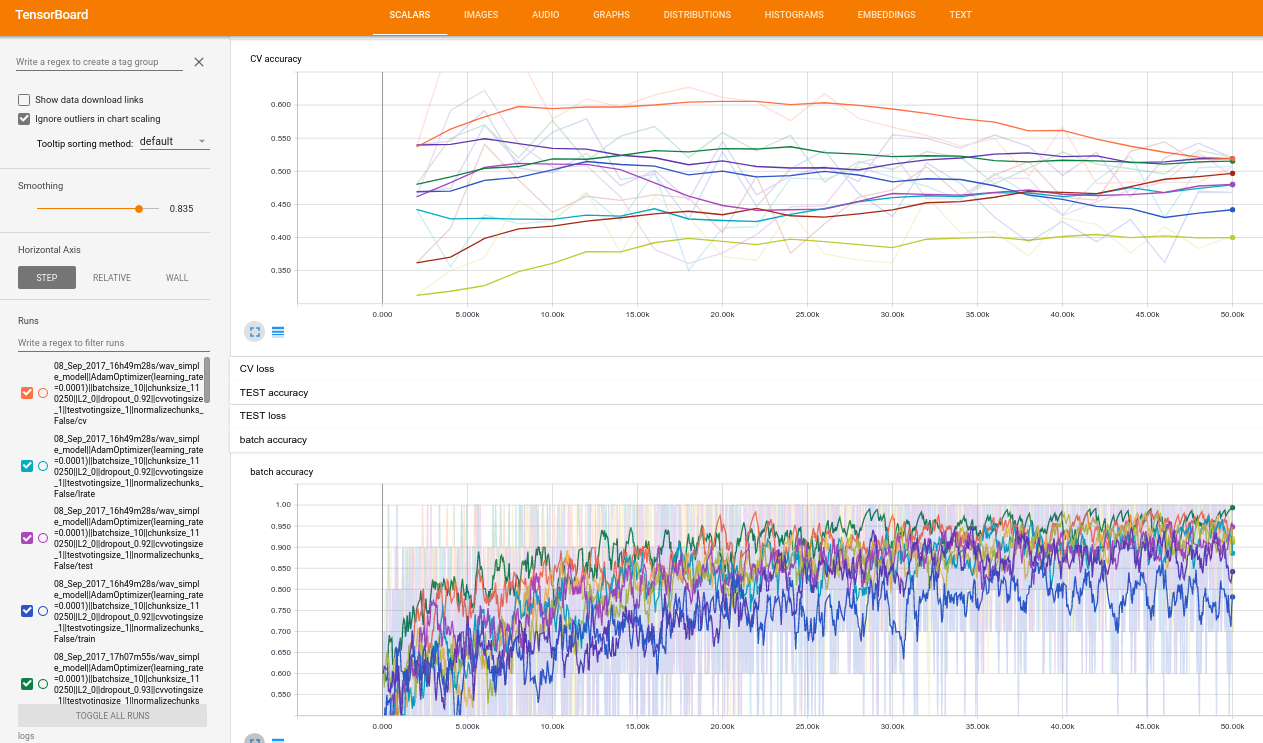
\includegraphics[scale=0.33]{tb_overfit.png}
  \caption{The validation (above) and batch (below) accuracy for many different models tested on two classes of the \(RRD^*\) dataset.}
  \label{fig:tb-overfit}
\end{figure}




\begin{figure}
  \centering
  \begin{subfigure}[b]{0.48\textwidth}
    \centering
    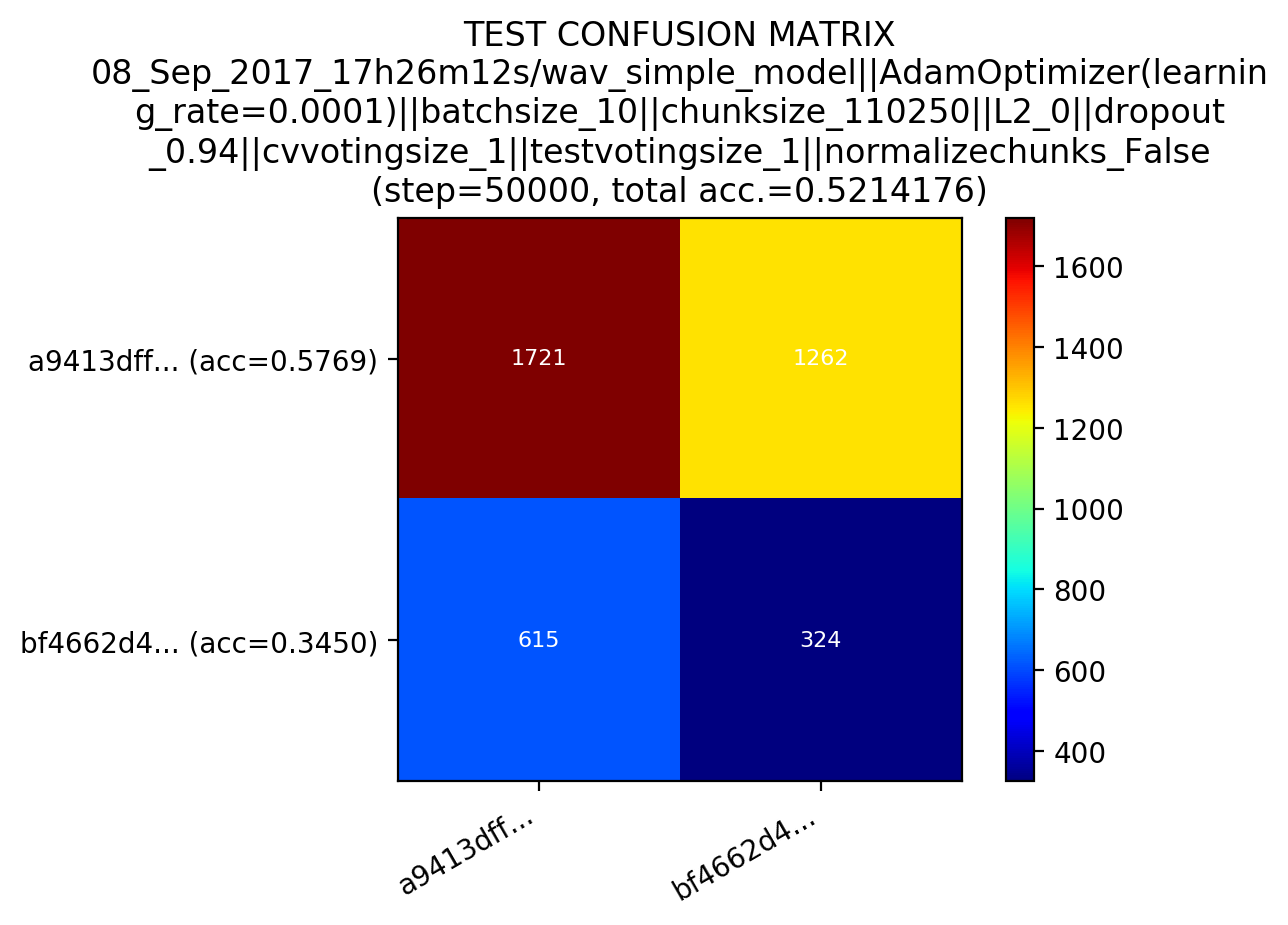
\includegraphics[width=\textwidth]{confmat1.png}
  \end{subfigure}
  \hfill
  \begin{subfigure}[b]{0.48\textwidth}
    \centering
    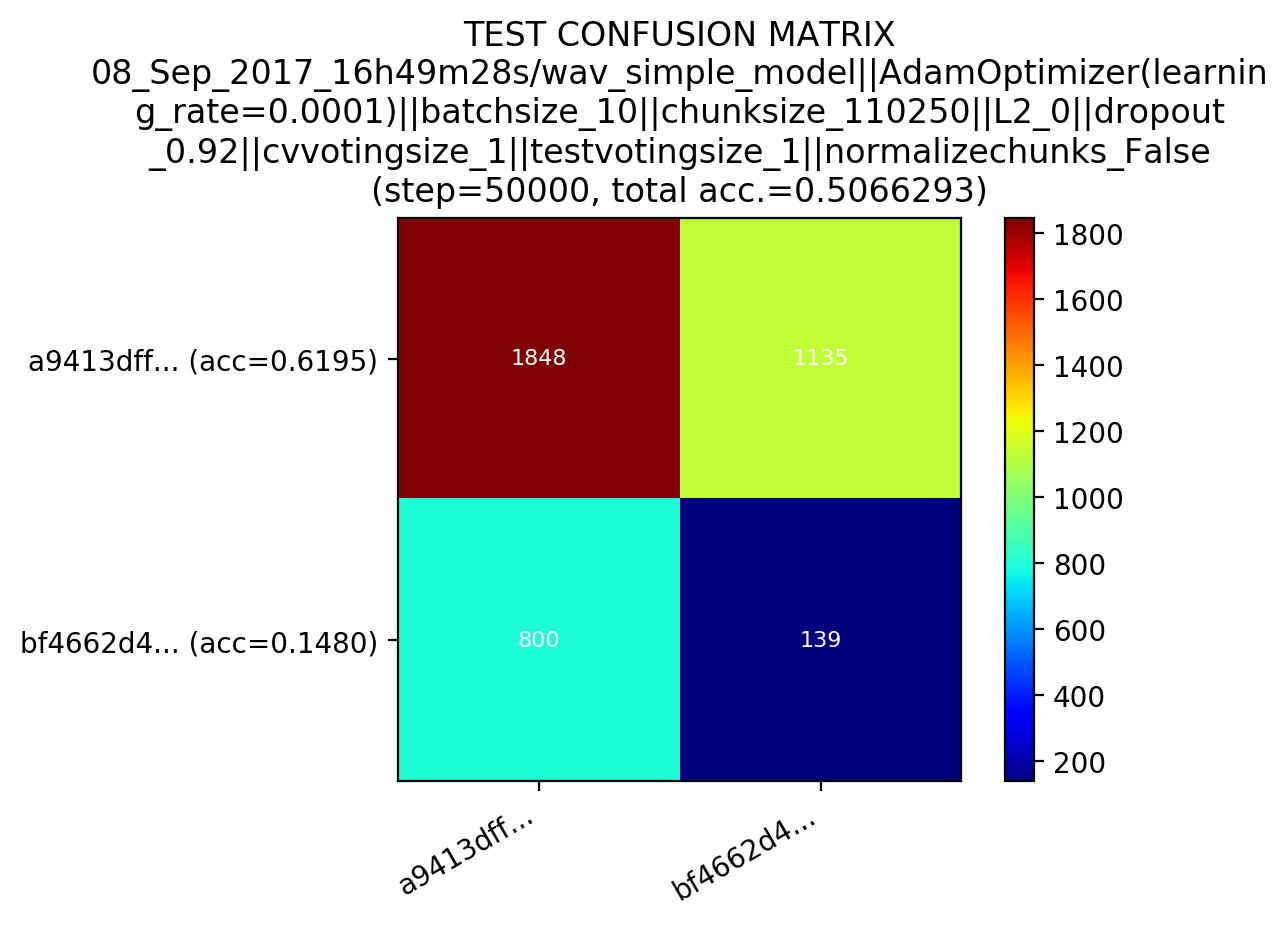
\includegraphics[width=\textwidth]{confmat2.png}
  \end{subfigure}
  \hfill
  \caption{The confusion matrices for two different models tested on two classes of the \(RRD^*\) dataset.}
  \label{fig:confmatrices}
\end{figure}
